\section{Results}
\label{sec:results}

\subsection{Area measurements}
Area measurements obtained using color blob detection/segmentation in \Matlab\ are shown in \fref{tab:results:area}.
\begin{table}
\caption{Area normal to flow for \Cxparadisi\ specimen and rigid physical model of a single grapefruit leaf.}
\label{tab:results:area}
\begin{center}
\begin{tabular}{cc}
\toprule
& area, \si{\meter\squared} \\
\midrule
\Cxparadisi\ grapefruit specimen & 0.223 \\
rigid physical model of leaf (metal) & 0.0346 \\
\bottomrule
\end{tabular}
\end{center}
\end{table}






\subsection{Drag measurements}
\Fref{tab:results:displacement} gives the measured raw displacement data for the \Cxparadisi\ specimen and the rigid physical model of a single grapefruit leaf. The resulting drag estimates are summarized in \fref{tab:results:drag} and figures~\ref{fig:results:drag} and \ref{fig:results:dragarea}. \Fref{fig:results:drag} shows... (what does it show). When the drag is normalized by area, the effect of leaf flexibility is apparent. \Fref{fig:results:dragarea} shows... (what does it show). 

\begin{table}
\caption{Measured raw displacement (\si{\meter}) for \Cxparadisi\ grapefruit specimen and rigid physical model of a single leaf (metal).}
\label{tab:results:displacement}
\begin{center}
\begin{tabular}{cccc}
\toprule
grapefruit & grapefruit & grapefruit & metal leaf \\
speed 1 & speed 2 & speed 3 & speed 3 \\ 
\midrule
%0.156 & 0.250 & 0.313 & 0.200 \\ % inches / cm 
%0.188 & 0.188 & 0.250 & 0.0500 \\
%0.250 & 0.250 & 0.313 & 0.100 \\
%0.188 & 0.219 & 0.313 & 0.200 \\
%0.188 & 0.250 & 0.313 & 0.150 \\
0.00397 & 0.00635 & 0.00794 & 0.00200 \\ % convert all to SI units
0.00476 & 0.00476 & 0.00635 & 0.00050 \\
0.00635 & 0.00635 & 0.00794 & 0.00100 \\
0.00476 & 0.00556 & 0.00794 & 0.00200 \\
0.00476 & 0.00635 & 0.00794 & 0.00150 \\
\bottomrule
\end{tabular}
\end{center}
\end{table}

\begin{table}
\caption{Summary of drag estimates for \Cxparadisi\ grapefruit specimen and rigid physical model of a single leaf (metal).}
\label{tab:results:drag}
\begin{center}
\begin{tabular}{lcccc}
\toprule
& grapefruit & grapefruit & grapefruit & metal leaf \\
& speed 1 & speed 2 & speed 3 & speed 3 \\
\midrule
drag, \si{\newton} & \num{0.051\pm0.008} & \num{0.061\pm0.007} & \num{0.079\pm0.007} & \num{0.014\pm0.007} \\
drag/area, \si{\newton\per\meter\squared} & \num{2.4\pm0.4} & \num{2.9\pm0.3} & \num{3.7\pm0.3} & \num{4.5\pm2.1} \\
\bottomrule
\end{tabular}
\end{center}
\end{table}

\begin{figure}
\begin{center}
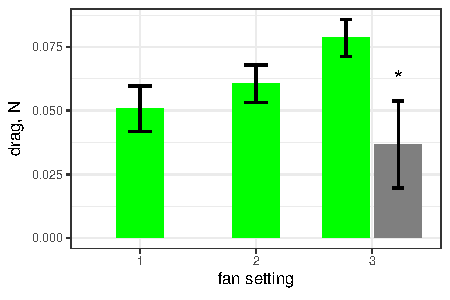
\includegraphics{data/results1.pdf}
\end{center}
\caption{Drag (mean$\pm$sd) for \Cxparadisi\ grapefruit specimen (green) and metal rigid physical model (gray) at different fan speeds. The rigid physical model leaf has less drag than the intact \Cxparadisi\ specimen because of smaller area (two-way ANOVA, $p<\num{4.6e-10}$, $n=5$).}
\label{fig:results:drag}
\end{figure}

\begin{figure}
\begin{center}
\includegraphics{data/results2.pdf}
\end{center}
\caption{Drag, normalized by area, (mean$\pm$sd) for \Cxparadisi\ grapefruit specimen (green) and metal rigid physical model (gray) leaves at different fan speeds. Normalized by area, the rigid metal leaf 19\% more drag than the flexible grapefruit leaves at the same speed, however, the differences are not statistically significant consider the small number of replicates and measurement noise (two-way ANOVA, $p=0.3207$, $n=5$). Differences in drag on the \Cxparadisi\ specimen are apparent at different speeds ($p=0.025$).}
\label{fig:results:dragarea}
\end{figure}






\subsection{Leaf movement during flow}
% This bit needs some help. 
\Fref{fig:results:leafmovement} shows frames from the slow motion video of \Cxparadisi\ at fan speed 3. Following the leaves indicated by the number 1, the leaves which were struck head-on by the wind flexed quite far at their joints, exposing roughly half of their surface area to the camera. The leaf indicated with the number 2 in \fref{fig:results:leafmovement} shows the continued vortex shedding on the leaves when wind was blown across them. The leaf pivoted at its joint, but only exposed about half of its area to the wind before returning to its previous state.
\begin{figure}
\begin{center}
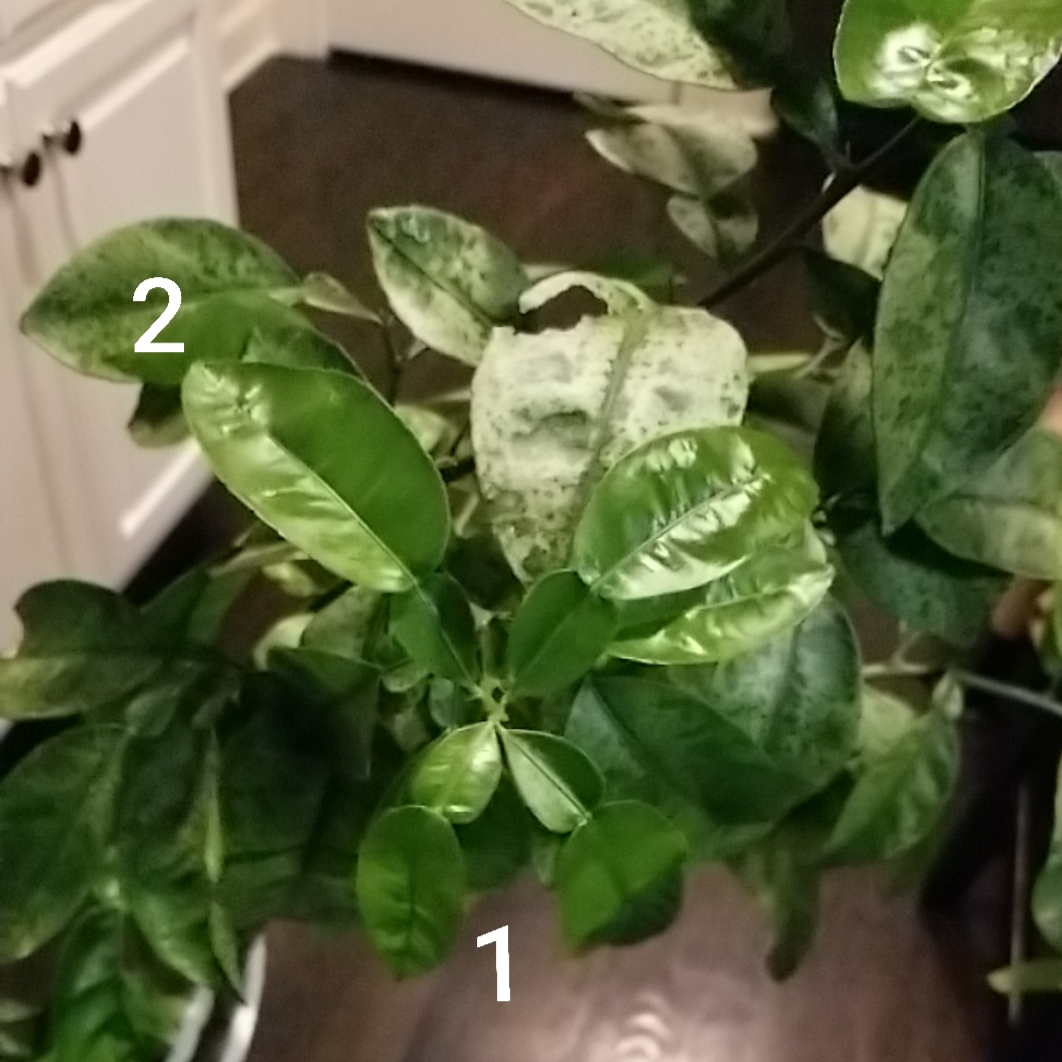
\includegraphics[width=0.49\columnwidth]{figures/Snapshot1.jpg}
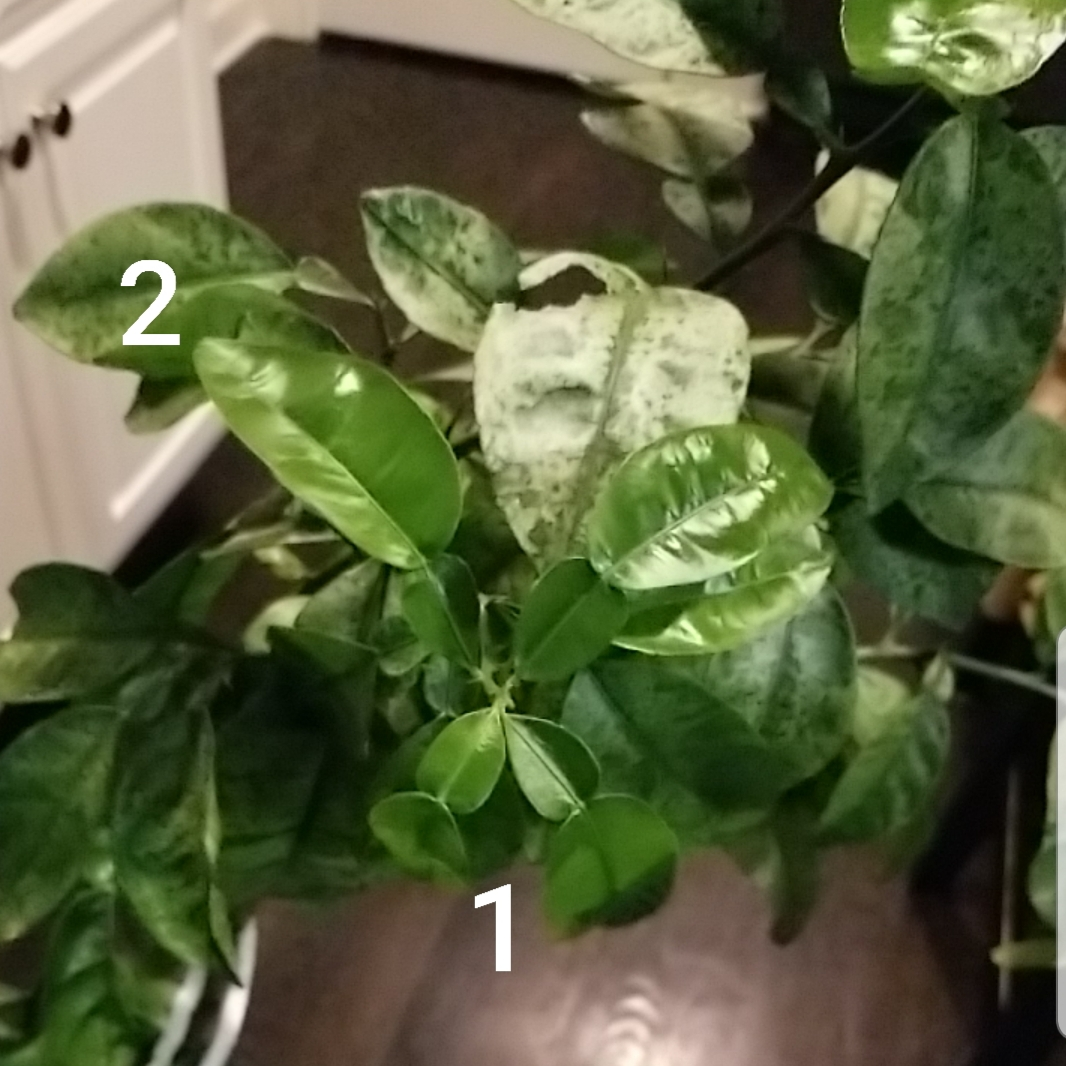
\includegraphics[width=0.49\columnwidth]{figures/Snapshot2.jpg}\\
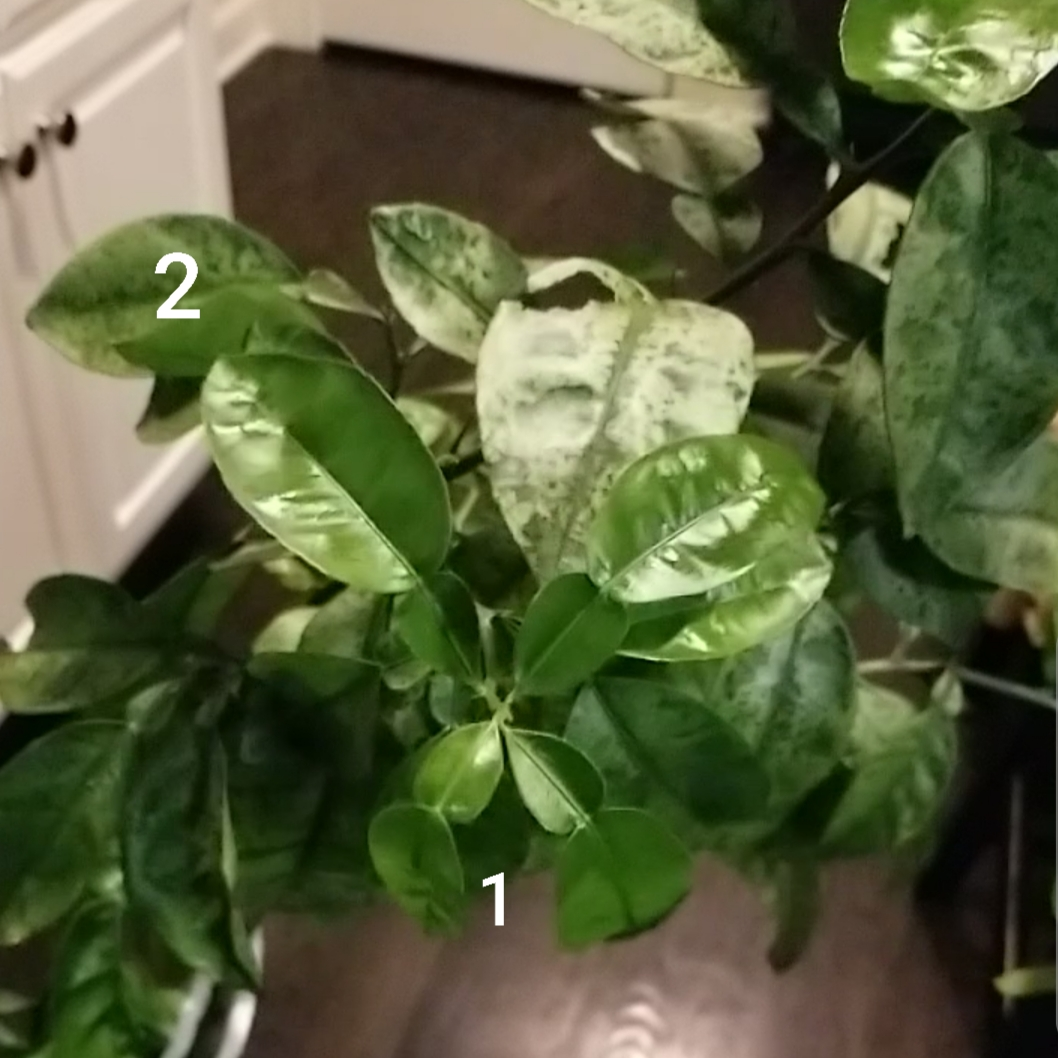
\includegraphics[width=0.49\columnwidth]{figures/Snapshot3.jpg}
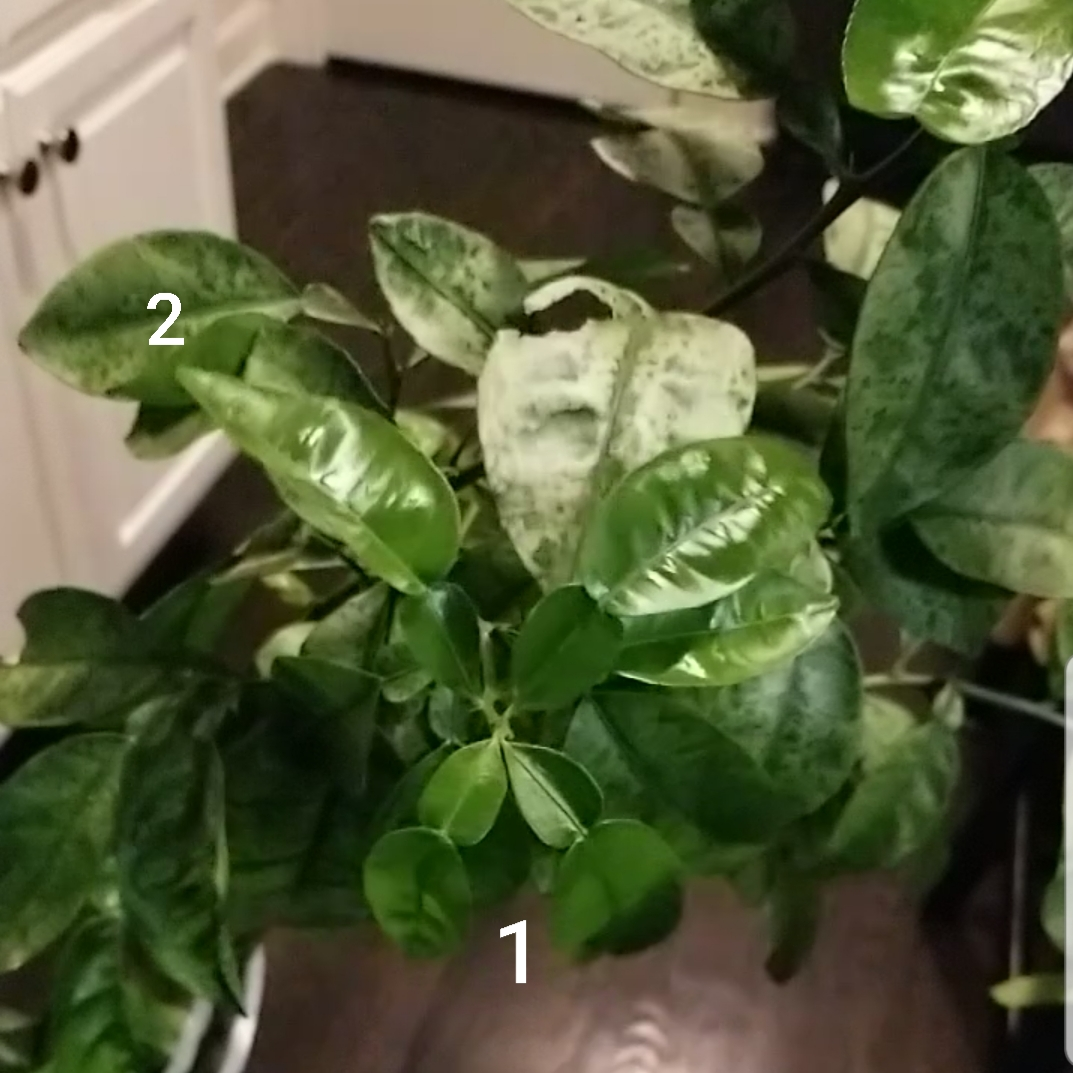
\includegraphics[width=0.49\columnwidth]{figures/Snapshot4.jpg}
\end{center}
\caption{Example frames from slow motion video of \Cxparadisi\ specimen at fan speed 3. Leaves marked 1 and 2 rotate at the petiole, reducing by half their area normal to the flow.}
\label{fig:results:leafmovement}
\end{figure}

